% ============================================================
% Conteúdo acadêmico puro do documento "Diagrama de Implantação".
% SEM \documentclass, \begin{document}/\end{document} nem título —
% pensado para ser reaproveitado via \input{} tanto no documento
% modular quanto, futuramente, no TCC principal.
%
% Fonte do conteúdo: Implantacao_RadarTorres.puml (nesta mesma
% pasta) e leitura direta do código-fonte/documentação técnica
% (README.md, Docs/Tecnica/COMUNICACAO_ARDUINO.md,
% installer/RadarTorres.iss) para confirmar nós, artefatos e
% protocolo de comunicação.
% ============================================================

\section{Apresentação}

Este documento especifica o diagrama de implantação do sistema \textbf{RadarTorres}, descrevendo
a distribuição física dos componentes de software sobre os nós de hardware envolvidos: o
computador do usuário, onde roda a aplicação desktop, e o Arduino, responsável pela leitura dos
sensores e pelo acionamento das torres demonstrativas. Serve de complemento ao \emph{Diagrama de
Classes} e ao \emph{Modelo de Banco de Dados} (estrutura estática e persistência), mostrando onde
cada parte do sistema efetivamente executa e como os nós se comunicam.

O sistema não possui nenhum componente de servidor, web ou nuvem: trata-se de uma aplicação
desktop única e autocontida, que se comunica com um único microcontrolador externo via porta
serial.

\section{Nós e Artefatos}

\begin{longtable}{p{3.6cm}p{3.0cm}p{7.4cm}}
  \caption{Nós e artefatos do diagrama de implantação} \\
  \hline
  \textbf{Nó} & \textbf{Tipo} & \textbf{Artefatos / Descrição} \\
  \hline
  \endfirsthead
  \multicolumn{3}{c}{\small \tablename~\thetable\ (continuação)} \\
  \hline
  \textbf{Nó} & \textbf{Tipo} & \textbf{Artefatos / Descrição} \\
  \hline
  \endhead
  \hline
  \endfoot
  \small
  Computador do usuário (Windows 10/11, 64-bit) & \texttt{node} & \texttt{RadarTorres.App}
  (C\# 13 / WPF, MVVM); \texttt{.NET 9 Desktop Runtime} embutido (instalação self-contained,
  via \texttt{installer/RadarTorres.iss}); armazenamento local em
  \texttt{\%AppData\%\textbackslash RadarTorres\textbackslash Data\textbackslash *.csv} (usuários,
  auditoria, objetos detectados, histórico de modos) e
  \texttt{\%LocalAppData\%\textbackslash RadarTorres\textbackslash *.json} (layout, preferências,
  zonas mortas). \\
  Arduino (microcontrolador) & \texttt{node} & Firmware responsável pela leitura dos sensores de
  ângulo/distância e pelo acionamento das torres demonstrativas. \\
  Sensores de detecção & \texttt{node} & Sensores de ângulo e distância que alimentam o Arduino
  com sinal analógico/digital. \\
  Torres demonstrativas / indicador & \texttt{node} & Laser de baixa potência ou LED, acionado
  pelo Arduino como resposta demonstrativa em modo Vermelho. \\
\end{longtable}

\section{Diagrama de Implantação}

O diagrama representa a aplicação desktop (\texttt{RadarTorres.App}) executando sobre o
\texttt{.NET 9 Desktop Runtime} no computador do usuário, sem depender de nenhum servidor
remoto. A comunicação com o Arduino ocorre via USB/Serial, usando um protocolo textual do tipo
\texttt{TIPO;CHAVE=VALOR;\ldots}. Fonte: \texttt{Implantacao\_RadarTorres.puml} (PlantUML), nesta
mesma pasta.

\begin{figure}[htbp]
  \centering
  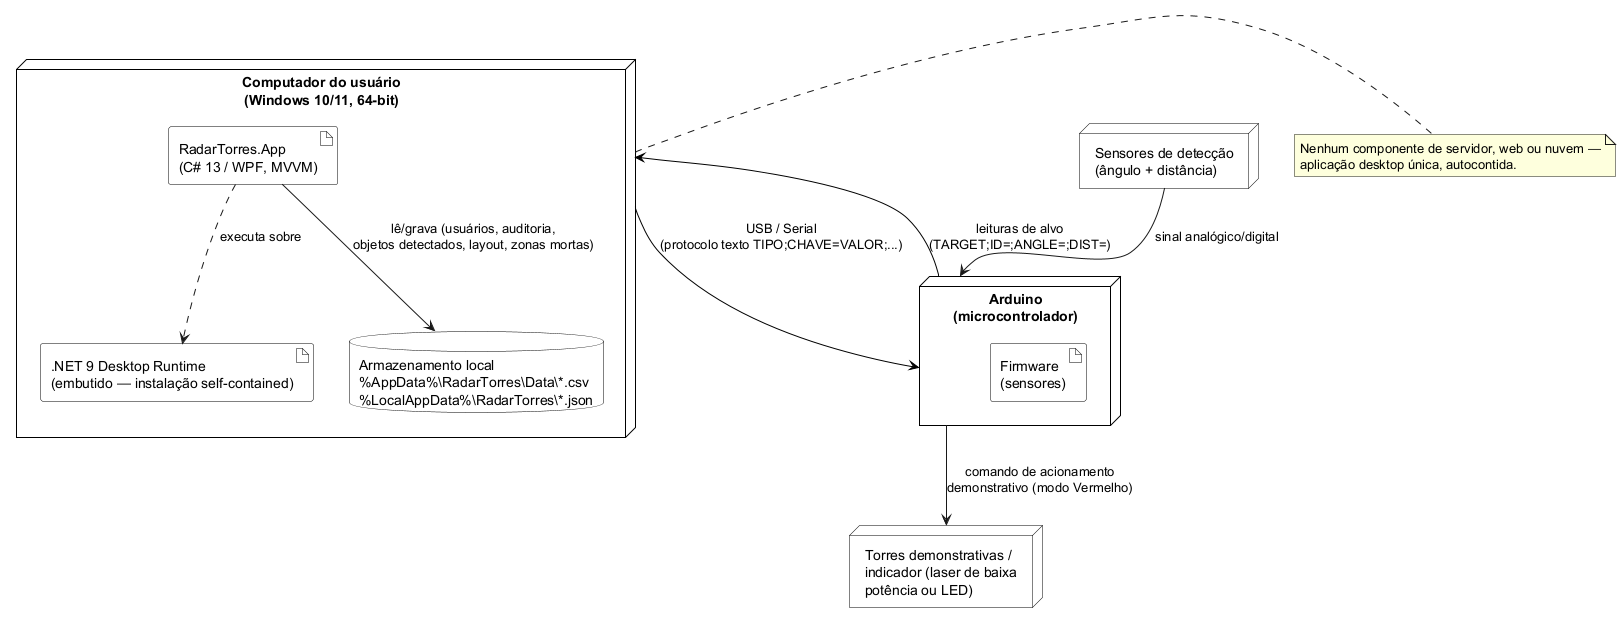
\includegraphics[width=\textwidth]{Implantacao_RadarTorres.png}
  \caption{Diagrama de implantação do RadarTorres.}
  \label{fig:implantacao}
\end{figure}

\section{Comunicação entre Nós}

\begin{longtable}{p{4.2cm}p{4.2cm}p{5.6cm}}
  \caption{Fluxos de comunicação entre nós} \\
  \hline
  \textbf{Origem} & \textbf{Destino} & \textbf{Descrição} \\
  \hline
  \endfirsthead
  \multicolumn{3}{c}{\small \tablename~\thetable\ (continuação)} \\
  \hline
  \textbf{Origem} & \textbf{Destino} & \textbf{Descrição} \\
  \hline
  \endhead
  \hline
  \endfoot
  \small
  Computador do usuário & Arduino & USB/Serial --- envio de comandos no protocolo texto
  \texttt{TIPO;CHAVE=VALOR;\ldots} (ex.: alteração de modo de operação). \\
  Arduino & Computador do usuário & USB/Serial --- leituras de alvo no formato
  \texttt{TARGET;ID=;ANGLE=;DIST=}. \\
  Sensores de detecção & Arduino & Sinal analógico/digital de ângulo e distância. \\
  Arduino & Torres demonstrativas & Comando de acionamento demonstrativo (modo Vermelho). \\
  RadarTorres.App & Armazenamento local & Leitura/gravação de usuários, auditoria, objetos
  detectados, layout e zonas mortas (arquivos CSV/JSON locais). \\
\end{longtable}

\section{Conclusão}

O diagrama de implantação evidencia a natureza autocontida do RadarTorres: um único nó de
software (a aplicação desktop, self-contained sobre o .NET 9) comunicando-se com um único
microcontrolador externo via porta serial, sem qualquer dependência de infraestrutura de
servidor, web ou nuvem. Toda a persistência ocorre localmente, no próprio computador do usuário,
o que simplifica a implantação a uma simples instalação via instalador (Inno Setup) na máquina
onde o sistema será operado.
